\documentclass[11pt]{article}
\usepackage[T1]{fontenc}
\usepackage[utf8]{inputenc}
\usepackage{times}
\usepackage{eurosym}
\usepackage{inconsolata}
\usepackage{amsmath}
\usepackage{framed}
\usepackage{graphicx}
\usepackage{hyperref}
\hypersetup{colorlinks=true, linkcolor=blue, urlcolor=blue}
\usepackage[usenames,dvipsnames,svgnames,table]{xcolor}
\definecolor{entityColor}{RGB}{0,100,200}
\definecolor{attributeColor}{RGB}{0,100,50}
\definecolor{relationColor}{RGB}{160,0,30}
\usepackage{listings}
\lstdefinestyle{reqT}{
  belowcaptionskip=1\baselineskip,
  breaklines=true,
  showstringspaces=false,
  basicstyle=\footnotesize\ttfamily,
  emph={Ent,Meta,Item,Label,Section,Term,Actor,App,Component,Domain,Module,Product,Release,Resource,Risk,Service,Stakeholder,System,User,Class,Data,Input,Member,Output,Relationship,Design,Screen,MockUp,Function,Interface,Epic,Feature,Goal,Idea,Issue,Req,Ticket,WorkPackage,Breakpoint,Barrier,Quality,Target,Scenario,Task,Test,Story,UseCase,VariationPoint,Variant},
  emphstyle=\bfseries\color{entityColor},
  emph={[2]has,is,superOf,binds,deprecates,excludes,helps,hurts,impacts,implements,interactsWith,precedes,requires,relatesTo,verifies},
  emphstyle={[2]\bfseries\color{relationColor}},
  emph={[3]Attr,Code,Constraints,Comment,Deprecated,Example,Expectation,FileName,Gist,Image,Spec,Text,Title,Why,Benefit,Capacity,Cost,Damage,Frequency,Min,Max,Order,Prio,Probability,Profit,Value,Status},
  emphstyle={[3]\color{attributeColor}},  
}
\lstset{style=reqT}
\usepackage{fancyvrb}
\usepackage[english]{babel}
\usepackage{blindtext}
\usepackage{enumitem} 
\setlist[itemize]{noitemsep}
\title{{\bf LAB 2:\\Requirements Prioritization \& Release Planning}\\ Instructions
}
\author{Björn Regnell}
\date{\today}
\begin{document}
\maketitle

\section{Introduction}

\subsection{Purpose} This document provides instructions on how to run 
a lab session on computer-supported requirements prioritization and release planning. Based on experiences from manually solving prioritization and release planning problems in your previous preparations, you will with this lab session gain insight into the benefits and limitations of using computer-aided constraint-based solving. 

\subsection{Prerequisites} This lab assumes that you have installed the open source tool \href{http://reqT.org}{reqT.org} and that you are familiar with basic requirements modeling using reqT. It is also assumed that you have completed \href{https://github.com/reqT/reqT/raw/3.0.x/doc/lab1/lab1.pdf}{Lab 1 Requirements Modeling}. You should also complete the preparations for Lab 2, available at \url{https://github.com/reqT/reqT/raw/3.0.x/doc/lab2/lab2.pdf} 

You should bring a file \verb+prio100.scala+ from the Lab 2 preparations to the lab computer. The file should include a reqT scala Model with at least two Stakeholder entities, each with a Prio attribute and a set of at least 15 Req entities each with a Benefit attribute.   

\subsection{How to plan your lab session?}
Devote approximately 25\% of your lab session time on Sections 2.1.1, 2.1.2, 2.2.1, and 2.2.2 respectively. If you get short of time, skip the {\it Extra if you are curious} steps.

\clearpage\newpage
\section{Instructions}\label{section:instr}

\subsection{Prioritization}


\subsubsection{Ratio scale prioritization}
In this section you will use reqT to calculate resulting priorities based your prepared \$100-method prioritization output. 
\begin{framed}
\noindent Do the following steps: 

\begin{enumerate}
\item Load your \verb+prio100.scala+ model into the tree in the reqT ModelTreeEditor.
\item Enter the following code in the reqT text editor. Similar code is available in the menu item:  Templates -> Prioritization \$100 Method.
\begin{lstlisting}
m =>    
val shs = m.entitiesOfType(Stakeholder)
val rs = m.entitiesOfType(Req)
val prioSum = shs.map(s => m/s/Prio).sum
val benefitSum = shs.map(s => 
  s -> (m/s).collect{ case Benefit(b) => b}.sum).toMap
val normalized = rs.map(r => 
  r has Benefit(
    math.round(shs.map(s => 
      (m/s/Prio)*(m/s/r/Benefit)*100.0 / (benefitSum(s)*prioSum)).sum).toInt)).toModel
println("\n--- Normalized, weighted priorities:\n" + normalized)
val sum = normalized.collect{ case Benefit(b) => b}.sum
println("\n--- Sum: " + sum)
println(normalized)
normalized.toString.save("prio100-result.scala")
m 
\end{lstlisting}
\item Apply the above function to the tree containing your prio100 model. Check the console for output and the contents of the output file \Verb+prio100-result.scala+.
\item What 5 requirements have the highest total normalized priority?
\vspace{4em}
\item Change the priorities of the stakeholders. How did the normalized requirements benefit change?
\vspace{3em}
%\item Use a web browser to navigate to the reqT source code at GitHub and in the source file in \verb+src/reqT+ named \verb+ModelBasicOps.scala+ search for ''\verb+def entitiesOfType+'' and explain what that method does. \newline a) What is the result type? \vspace{1em}\newline b) Can the collection include duplicate items? (Hint: search for ''\verb+lazy val entities+'' and check if the method \verb+distinct+ is applied or not.)
%\vspace{1em}
\item {\it Extra if you are curious:} Check the code in step 2 above and try to match the code to the calculations in the preparations Section 2.1.2. You can insert \verb+println+ of interesting values to better understand what they contain, e.g. \verb+println(benefitSum)+. Try to find which {\verb+val+} declarations in the above code that correspond to which sums in the formulas in the preparations. 
%\vspace{6em}
\item Open a spread sheet program (e.g. LibreOffice Calc or MS Excel) and create the column headings Stakeholder;Feature;Prio and fill in the columns similar to this, using your own priorities:
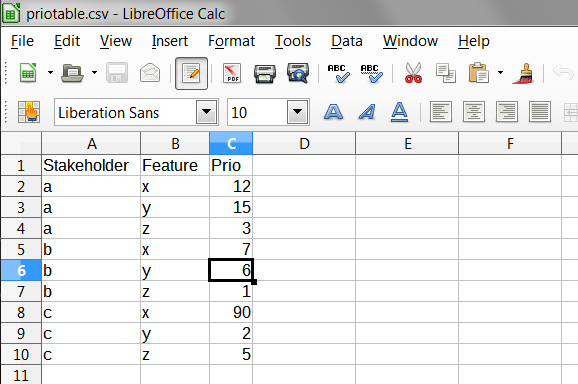
\includegraphics[width=0.9\textwidth]{spread-sheet.png}
\item Use Save As ... or Export and save your spread sheet in the .csv text file format, using semicolons as column separators (the default is depending on your locale). Open the file in a text editor and check that it has semicolons as column separators. Fix it if not, e.g. using your favorite editor's search-replace feature.
\item Select the Import -> From Prio Table menu item in the reqT gui, and import your spread sheet to the tree.
\item Add a Prio attribute to each stakeholder in the tree, using <Ctrl+E> and <Ctrl+R>, to model that stakeholders have different importance. 
\item Calculate the normalized total priorities using the code from step 2 above. The code might be available in your undo history, check with <Ctrl+Z> in the text editor pane of the reqT gui. Check that the calculations seems correct.
\item Discuss with a friend how you could use the Import -> From Prio Table feature of reqT when you elicit priorities in your project. How would you prepare the data collection from stakeholders? Write down your reflections.
\vspace{12em}
\item {\it Extra if you are curious:} Investigate the code in the reqT source file named \verb+parse.scala+ in the reqT repo at GitHub. How could you use the \verb+load+ method in \verb+ object Tab + to import a .csv file that have another character than semicolon as column separator? 
\end{enumerate}

\end{framed}
\newpage\clearpage
\subsubsection{Ordinal scale prioritization}

In this section you will use reqT to re-prioritize your features from the previous step, now with computer-supported ordinal scale prioritization. 
\begin{framed}
\noindent Do the following steps: 

\begin{enumerate}
\item Load your \verb+prio100.scala+ model into the tree in the reqT ModelTreeEditor. We will not use the values from the \$100-method -- we just need the requirement entities to generate pairwise combinations in a special text file, hence the code below starts with grabbing your Req entities. Enter the following code in the reqT text editor. Similar code is available in the menu item:  Templates -> Prioritization Ordinal Ranking.
\begin{lstlisting}
m => 
val rs = m.entitiesOfType(Req)
val pairs = scala.util.Random.shuffle(rs.combinations(2).toVector)
val rows = pairs.map{case Vector(p1,p2) => 
  s"${p1.id} <> ${p2.id}"}.mkString("\n")
println(rows)
val fileName = "prio-ord.txt"
rows.save(fileName)
val msg1 = s"Edit file $fileName in another editor\n"
val msg2 = "Change <> to either > or <\nto reflect your priorities."
val msg3 = "Press OK when you have saved your changes in a NEW file called prio.txt"
javax.swing.JOptionPane.showMessageDialog(null,msg1+msg2+msg3)
val edited = load("prio.txt")
val ranked = reqT.parse.comparisonParser.parseAndSolve(edited,allowedDeviation=0)
if (ranked!=Model()) edit(ranked) else 
  javax.swing.JOptionPane.showMessageDialog(null,"Inconsistent. See console.")
m
\end{lstlisting}
The above code invokes a constraint solver that uses comparisons as input and tries to find ranks that are consistent with all comparisons. If there are inconsistencies among the comparisons the  \verb+allowedDeviation+ parameter can be increased to tolerate a limited number of rank errors, and still calculate a solution.
\item Apply the above function to the tree containing your prio100 model. Edit the file prio-ord.txt outside reqT using your favorite editor when the JOptionPane occurs, and save your comparisons in another file called prio.txt. Try to be consistent. What are the 3 best-ranked requirements?
\vspace{1em}
\item Introduce some inconsistencies among your comparisons and try again. Increase \verb+allowedDeviation+ to some integer > 0. Observe the retries printed in the console window. (When you re-run the ranking solving, it is actually enough to run the part from when the comparisonParser is invoked and onwards.) How many times did the solver try before succeeding to produce a ranking when you increase the \verb+allowedDeviation+? How ''bad'' is the produced ranking in comparison to a ''correct'' ranking?
\vspace{4em}
\item It is difficult to be consistent if there are many requirements. What does it mean that a prioritizer is inconsistent in terms of that person's knowledge about priorities of the domain?
\vspace{4em}
\item If you think $n(n-1)/2$ are too many comparisons, how would you go about reducing them?
 \vspace{3em}
\item {\it Extra if you are curious:} Generate $n-1$ comparisons only by changing how the \verb+pairs+ variable is generated in the code of step 1 to:
\begin{lstlisting}
val pairs = for (i<- 0 until rs.size) yield 
    Vector(rs(i),rs((i+1) % rs.size)) 
\end{lstlisting}
\item {\it Extra if you are curious:} Read the code of the comparisonParser and try to figure out how the constraint problem is generated. \url{https://github.com/reqT/reqT/blob/3.0.x/src/reqT/parse.scala#L165} 
\end{enumerate}

\end{framed}

\clearpage\newpage

\subsection{Release Planning}
\subsubsection{Simple release planning}
In this section you will investigate use reqT to do release planning using a simple model with just a few features. 
\begin{framed}
\noindent Do the following steps: 

\begin{enumerate}
\item Enter the following code in the reqT gui text editor by choosing the menu item ''Templates -> Release planning example, simple''.

\begin{lstlisting}
val simple = Model(
  Stakeholder("X") has (
    Prio(1),
    Feature("1") has Benefit(4),
    Feature("2") has Benefit(2),
    Feature("3") has Benefit(1)),
  Stakeholder("Y") has (
    Prio(2),
    Feature("1") has Benefit(2),
    Feature("2") has Benefit(1),
    Feature("3") has Benefit(1)),
  Release("A") precedes Release("B"),  
  Resource("dev") has (
    Feature("1") has Cost(10),
    Feature("2") has Cost(70),
    Feature("3") has Cost(40),
    Release("A") has Capacity(100),
    Release("B") has Capacity(100)),
  Resource("test") has (
    Feature("1") has Cost(40),
    Feature("2") has Cost(10),
    Feature("3") has Cost(70),
    Release("A") has Capacity(100),
    Release("B") has Capacity(100)),
  Feature("3") precedes Feature("1"))
val problem = csp.releasePlan(simple)
val solution = problem.maximize(Release("A")/Benefit)
val sortedSolution = solution.
  sortByTypes(Release, Feature, Stakeholder, Resource)
sortedSolution
\end{lstlisting}
\item Load the \verb+sortedSolution+ model into the tree by selecting the tree root and run the above code using <Ctrl+R>. 
\item Investigate the solution in the tree and write down which features that have been allocated to releases A and B respectively:
\newline Features of release A:
\vspace{1em}
\newline Features of release B:
\vspace{1em}
\item Run the code from step 1 again but now using <Ctrl+Enter> and then type this code in the reqT console:
\begin{lstlisting}
(problem/Constraints).foreach(println)
\end{lstlisting}
\item Try to find the constraint in the above printed listing that models the ordering of releases and write down the constraint here:
\vspace{1.5em}
\item Try to find the precedence constraint that models the precedes relation \newline\lstinline+Feature("3")  precedes  Feature("1")+ and write down the constraint here:
\vspace{1.5em}
\item Inspect the other constraints in the console listing from step 4 and try to relate some of them to the formulas of the definition of the release planning problem in the preparations.
\item Change the problem in various ways, e.g. remove the precedes relation, change capacities and priorities etc. What happens if the problem has no solution?
\vspace{1em}
\item {\it Extra if you are curious:} Check out the code that generates the release planning constraint problem at \url{https://github.com/reqT/reqT/blob/3.0.x/src/reqT/csp.scala} and try to find some code lines that correspond to the definition of the release planning problem in the preparations. 

Sometimes it takes very long to find a solution. The constraint solving process can be given a time out and other parameters to control the search. Look at this code to investigate opportunities of controlling the solution search: \url{https://github.com/reqT/reqT/blob/3.0.x/src/reqT/jacop.scala#L38} The SearchType trait is available here: \url{https://github.com/reqT/reqT/blob/3.0.x/src/reqT/constraints.scala#L88} 
\end{enumerate}

\end{framed}

\subsubsection{Advanced release planning}
\begin{framed}
\noindent Do the following steps: 

\begin{enumerate}
\item Enter the following code in the reqT gui text editor by choosing the menu item ''Templates -> Release planning example, advanced''.

\begin{lstlisting}
val m = Model(
  Resource("TeamA") has (
    Feature("exportHtml") has Cost(9),
    Feature("exportGraphViz") has Cost(7),
    Feature("exportTabular") has Cost(3),
    Feature("exportLatex") has Cost(6),
    Feature("exportContexDiagramSvg") has Cost(3),    
    Feature("syntaxColoring") has Cost(6),
    Feature("autoCompletion") has Cost(3),    
    Feature("releasePlanning") has Cost(4),    
    Feature("autoSave") has Cost(6),    
    Release("March") has Capacity(20),
    Release("July") has Capacity(15),
    Release("later") has Capacity(1000)),
  Resource("TeamB") has (
    Feature("exportHtml") has Cost(2),
    Feature("exportGraphViz") has Cost(8),
    Feature("exportTabular") has Cost(9),
    Feature("exportLatex") has Cost(4),
    Feature("exportContexDiagramSvg") has Cost(4),
    Feature("syntaxColoring") has Cost(2),    
    Feature("autoCompletion") has Cost(3),    
    Feature("releasePlanning") has Cost(5),    
    Feature("autoSave") has Cost(7),    
    Release("March") has Capacity(15),
    Release("July") has Capacity(15),
    Release("later") has Capacity(1000)),
  Release("March") has Order(1),
  Release("July") has Order(2),
  Release("later") has Order(3),
  Stakeholder("Ada") has (Prio(1), 
    Feature("exportHtml") has Benefit(10),
    Feature("exportGraphViz") has Benefit(10),
    Feature("exportTabular") has Benefit(10),
    Feature("exportLatex") has Benefit(7),
    Feature("exportContexDiagramSvg") has Benefit(6),
    Feature("syntaxColoring") has Benefit(3),    
    Feature("releasePlanning") has Benefit(4),    
    Feature("autoCompletion") has Benefit(7),    
    Feature("autoSave") has Benefit(9)))
val solution = csp.releasePlan(m).
    maximize(Release("March")/Benefit).
    sortByTypes(Release, Feature, Stakeholder, Resource)
solution
\end{lstlisting}

\item Press <Ctrl+R> to replace the tree root with the solution. Use the menu item ''Tree -> Collapse all'' and the inspect parts of the tree to see the allocated features. Press <Ctrl+R> again and investigate if the solution found is the same each time?

\item Investigate which features were allocated to release March with the code below. Compare to your manual solution from the preparations. How close to optimal were you able to get?

\begin{lstlisting}
m =>
  val march = (m/Release("March") - Resource).atoms.
    collect{
      case Relation(e,l,Model(Benefit(i))) if i >0 => 
        (e.id,i)
    }
   println(march.mkString("\n"))
   println("SUM: " + march.collect{case (s,b) => b}.sum)
m  
\end{lstlisting}
\item Add the precedes relation (un-comment code in template) 
\newline\lstinline+ Feature("exportHtml")   precedes Feature("exportGraphViz")+ \newline and explain how  it impacts the allocation.  
\item Add another stakeholder (uncomment code in template) and explain how it impacts the allocation.
\begin{lstlisting}
Stakeholder("Ben") has (Prio(1), 
    Feature("exportHtml") has Benefit(1),
    Feature("exportGraphViz") has Benefit(9),
    Feature("exportTabular") has Benefit(3),
    Feature("exportLatex") has Benefit(4),
    Feature("exportContexDiagramSvg") has Benefit(7),
    Feature("syntaxColoring") has Benefit(8),    
    Feature("releasePlanning") has Benefit(5),    
    Feature("autoCompletion") has Benefit(10),    
    Feature("autoSave") has Benefit(4)) 
\end{lstlisting}   
\item What is the lowest capacities of each resource that you can allocate in order for a solution to still exist?
\vspace{1.5em}
\item {\it Extra if you are curious:} Investigate the generated constraints of an 'advanced' problem with both precedence constraints and multiple stakeholders, by using the code template from step 1, uncommenting precedes and the second stakeholder, and by changing the last part of the code in step 1 to:
\begin{lstlisting}
val problem = csp.releasePlan(m)
(problem/Constraints).foreach(println)
println("Number of constraints:" + (problem/Constraints).size)
val solution = problem.maximize(Release("March")/Benefit)
val sortedSolution = solution.
  sortByTypes(Release, Feature, Stakeholder, Resource)
sortedSolution
\end{lstlisting}   
How many constraints were generated?
How is the \verb+IfThenElse+ constraint used to allocate features?
\item Discuss with a friend how you can conduct release planning in your project using constraint solving. Which requirements should be included in the release plan? Which stakeholders should be allowed to impact the decisions? How will you represent the release planing input data? Write down your reflections.
\vspace{22em}
\end{enumerate}

\end{framed}
\end{document}
